\chapter{Introduction}\label{chap:chapter1}

\epigraph{\myopeningquote Our greatest glory is not in never falling, but in rising every time we fall.\myclosingquote}
{Confucius}%



Unification of Quantum Mechanics and General Relativity has been the Holy Grail of physics for since their inception. But no satisfactory theory has ever been proposed that solves this problem? General relativity states that a physical theory should not depend on background structures. However, standard quantization techniques often rely on background structures, such as imposing the canonical commutation relations. The Hamiltonian of a generally covariant theory, such as general relativity, is constrained to vanish in the absence of boundaries. If one tries to incorporate the theory of general relativity and quantum mechanics i.e in Canonical Quantization of gravity one ends up with a Hamiltonian constraint (i.e. \(\Hat{\operatorname{\mathbf{H}}}\left|\Psi\right\rAngle = 0\)). This leads to an infamous problem known as ``the problem of time” in the canonical approach to quantum gravity. The issue is that quantum states of spacetime (and matter in it) do not seem to undergo any time evolution as dictated by the constraints of the theory.
\section{Example Section}\label{sec:example_section}
Include equations if required:
%%%
% Example Equation.

\begin{equation}
\label{eq:straight_line}
i\hbar \frac{\partial \Psi}{\partial t} = -\frac{\hbar^2}{2m} \nabla^2 \Psi + \hat{V}\Psi
\end{equation}
\[
\nabla \times \mat{B} = \mu_0 \mat{J} + \mu_0 \varepsilon_0 \frac{\partial \mat{E}}{\partial t}
\]

%%%

The issue is that quantum states~\cite{article_name} of spacetime (and matter in it) do not seem to undergo any time evolution as dictated by the constraints of the theory.
\begin{Frame}[Frame Title]
However, upon closer inspection, it is clear that the quantum theory is not 'timeless' as often stated. The problem of time is rather a manifestation of background independence and means that physical states do not evolve relative to an external background time. Instead, one must extract a time evolution in a relational manner, i.e. pick some quantised degrees of freedom to serve as an internal time.
    \begin{equation}
\label{eq:glob_ham}
    H = \sum_{k = 0}^{N-1} H_k 	\equiv \sum_{k = 0}^{N-1} \hbar 
\omega_k \sigma_{z}^{(k)}
\end{equation} 
\end{Frame}
 The use of relational time in Quantum Mechanics is a framework in which one promotes all variables to Quantum operators and later chooses one of the variables to operate like a "clock". There are various approaches to the time problem; my work focuses on the "Page-Wootters Formalism" which defines relational dynamics in terms of conditional probabilities for the clock and evolving degrees of freedom.




Include figures if required:
%%%
% Example Figure.
\begin{figure}[ht!]
    \centering
    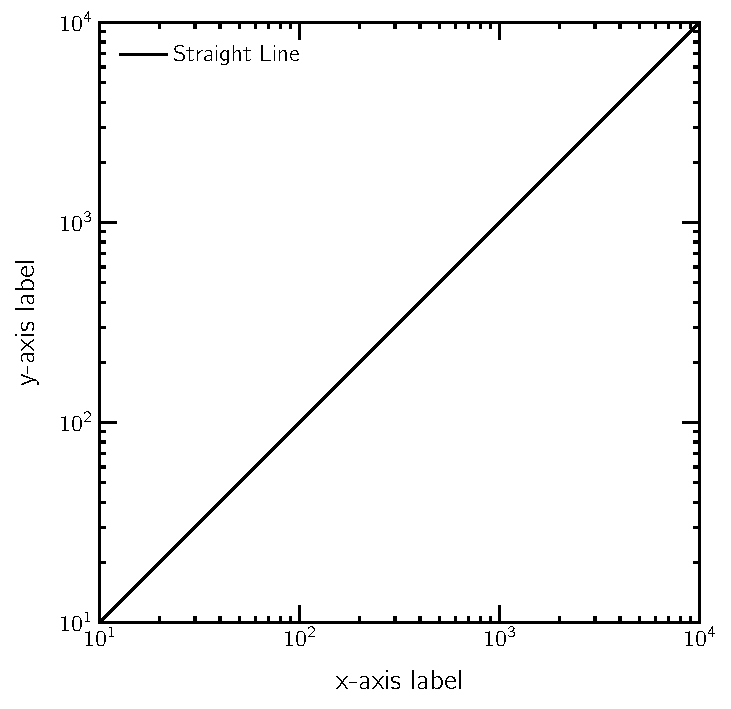
\includegraphics[width=8cm]{Chapter1/figure1.pdf}
    \caption{Example Figure: Include a caption.}
    \label{fig:example_figure}
\end{figure}
%%%

\newpage

Include tables if required:
%%%
% Example Table.
\begin{table}[ht!]
\centering
    \begin{tabular}{||c c c c||} 
     \hline
     Col1 & Col2 & Col2 & Col3 \\ [0.5ex] 
     \hline\hline
     1 & 2 & 3 & 4 \\ 
     \hline
     5 & 6 & 7 & 8 \\ 
     \hline
    \end{tabular}
\caption{Example Table: Include a caption.}
\label{table:example_table}
\end{table}
%%%

To refer to Equations/Figures/Tables, use the \verb!\ref{}! command: Equation~\ref{eq:straight_line} / Figure~\ref{fig:example_figure} / Table~\ref{table:example_table}. \verb!\ref{}! can also be used to refer to Sections: Section~\ref{sec:example_section}, Section~\ref{ssec:example_subsection}.

To cite references, use the \verb!\cite{}! command: \cite{article_name}. All cited references will automatically appear in the Bibliography section.

\subsection{Example Sub-Section}\label{ssec:example_subsection}

Create a sub-section if required.

\subsubsection{Example Sub-Sub-Section}\label{sssec:example_subsubsection}

Create a sub-sub-section if required.